\documentclass[10pt,a4paper]{article}
\usepackage[utf8]{inputenc}
\usepackage[english]{babel}
\usepackage{amsmath}
\usepackage{amsfonts}
\usepackage{amssymb}
\usepackage{graphicx}
\usepackage[left=2cm,right=2cm,top=2cm,bottom=2cm]{geometry}
\usepackage{physics}
\usepackage{tikz}
\usepackage{stmaryrd}

\author{Marco Biroli}
\title{Graphene and Haldane model}

\begin{document}

\maketitle

\section{Remark}

Throughout the homework I will use $f$ with the opposite sign convention:
\[
f_{\vb{k}} = -t \sum_j e^{i\vb{k} \cdot \vb{\delta_j}}
\]
This is due to the fact that if we use the sign convention as it is stated in the homework we will obtain:
\[
f_{\vb{K} + \vb{q}} = \frac{3 d t}{2}(q_x - iq_y)
\]
Which is incompatible with the notation used in questions 2.6 and onwards. With opposite sign convention however we do indeed obtain the result expected:
\[
f_{\vb{K} + \vb{q}} = \frac{3 d t}{2}(q_x + iq_y)
\]
Note that this changes nothing to the physics since it is simply equivalent to taking a transpose of the Hamiltonian. 

\section{Graphene and Dirac points.}

\begin{enumerate}
\item  We have that:
\[
\vb{\delta_1} = (0, a) \mbox{~~and~~} \vb{\delta_2} = \frac{d}{2} (\sqrt{3}, -1) \mbox{~~and~~} \vb{\delta_3} = \frac{d}{2} (-\sqrt{3}, -1)
\]
Then we have that:
\begin{align*}
f_{\vb{k}} &= t \left(-\left(e^{-\frac{1}{2} i d \left(\sqrt{3} \text{kx}-\text{ky}\right)}+e^{\frac{1}{2}
   i d \left(\sqrt{3} \text{kx}+\text{ky}\right)}+e^{-i d \text{ky}}\right)\right)\\
&= -t \left[
\underbrace{\left(2 \cos \left(\frac{1}{2} \sqrt{3} d \text{kx}\right) \cos \left(\frac{d
   \text{ky}}{2}\right)+\cos (d \text{ky})\right)}_{h_1} - i \underbrace{\left(\sin (d \text{ky})-2 \cos \left(\frac{1}{2} \sqrt{3} d \text{kx}\right) \sin
   \left(\frac{d \text{ky}}{2}\right)\right)}_{h_2}
\right]
\end{align*}
And taking $h_3 = 0$ we have that:
\[
H = -t \, \, \vb{h}_{\vb{k}} \cdot \vb{\sigma}
\]
Notice that without expanding the terms we can also simply write:
\[
H = \sum_{i = 1}^3 \left( \cos(\vb{k} \cdot \vb{\delta_i} ) \sigma_x + \sin(\vb{k} \cdot \vb{\delta_i}) \sigma_y \right)
\]
Then notice that similarly as in the TD we have that:
\[
H^2 = t^2 || \vb{h}_{\vb{k}} ||^2 \text{ Id}
\]
Thus the eigenvalues of $H$ are given by:
\[
E_\pm = \pm t || \vb{h_{\vb{k}}} || = \pm t \sqrt{3 + 2 \cos(d k_x \sqrt{3}) + 2 \cos(\frac{d}{2} (k_x\sqrt{3} - 3 k_y)) + 2 \cos(\frac{d}{2}(k_x\sqrt{3} + 3k_y))}
\]
Notice that solving for $E_\pm = 0$ we get indeed the Dirac point $K$, as well as $-K$ or $(K_x, - K_y)$ for example. Plotting the energy spectrum we obtain Figure \ref{eigenplot}.
\begin{figure}
\centering
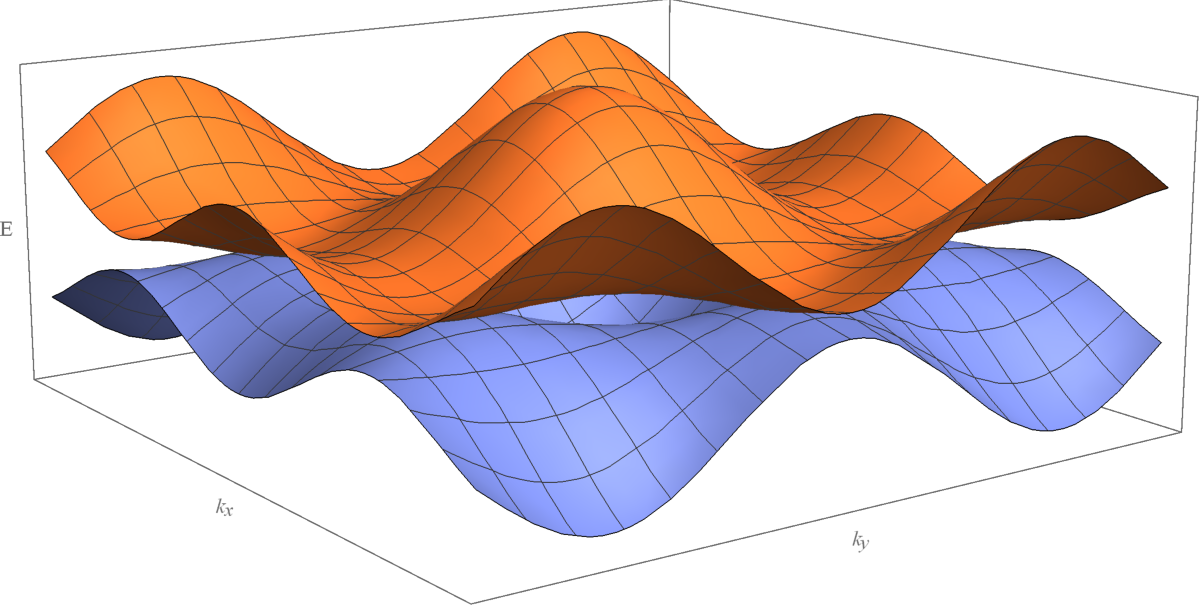
\includegraphics[width = 0.5\textwidth]{energylevels}
\caption{Plot of the positive energy levels for $d k_x, d k_y \in [-\pi, \pi]$. In orange the $E_+$ solution is represented and in blue the $E_-$ solution.} \label{eigenplot}
\end{figure}

\item We write $\vb{k} = \vb{K} + \vb{\varepsilon}$. Then we know that $H_{\vb{K}} = 0$ and $f_{\vb{K}} = 0$ hence we have that:
\[
f_{\vb{k}} = f_{\vb{K}}  + \vb{\varepsilon} \cdot \left(\grad f_{\vb{k}} \right) \Big|_{\vb{k} = \vb{K}} = \vb{\varepsilon} \cdot \left( \frac{3 d t}{2}, \frac{3}{2} i d t  \right) = \frac{3dt}{2}\left( \varepsilon_x + i \varepsilon_y \right)
\] 
Hence we also get the linearization of $\vb{h}$ easily as:
\[
\vb{h}_{\vb{k}} = \left(\frac{3dt}{2} (k_x - K_x), \frac{3 dt}{2} (k_y - K_y)\right)  = \frac{3 dt}{2}\left(\varepsilon_x,  \varepsilon_y \right)
\]
And hence:
\[
E_\pm = \pm t \frac{3 dt}{2} \sqrt{\varepsilon_x^2 + \varepsilon_y^2} = \pm \frac{3 d t}{2} r 
\]

\item Close to $\vb{K}$ the Hamitlonian reads:
\[
H = \frac{3 d t}{2}\begin{pmatrix}
0 & \varepsilon_x - i \varepsilon_y\\
\varepsilon_x + i \varepsilon_y & 0 
\end{pmatrix}
\]
Hence we have that the eigenvectors are given by:
\[
u_{\pm \vb{k}} = \begin{pmatrix}
\pm \sqrt{\varepsilon_x - i \varepsilon_y}\\
\sqrt{\varepsilon_x + i \varepsilon_y}
\end{pmatrix} = \begin{pmatrix}
\pm \sqrt{\varepsilon} e^{-i \theta/2}\\
\sqrt{\varepsilon} e^{i \theta/2} 
\end{pmatrix}
\]
Where we took:
\[
\cos \theta = \frac{\varepsilon_x}{\varepsilon} \mbox{~~and~~} \sin \theta = \frac{\varepsilon_y}{\varepsilon} \mbox{~~and~~} \varepsilon = \sqrt{\varepsilon_x^2 + \varepsilon_y^2}
\]
Then we have that:
\[
\pdv{}{\varepsilon_x} u_{\pm \vb{k}} = \pdv{}{\varepsilon} \pdv{\varepsilon}{\varepsilon_x} u_{\pm \vb{k}} + \pdv{}{\theta} \pdv{\theta}{\varepsilon_x} u_{\pm \vb{k}} = \frac{\cos\theta}{2 \sqrt{\varepsilon}} \begin{pmatrix}
\pm e^{-i\theta/2}\\
e^{i\theta/2}
\end{pmatrix}
- \frac{i \sin\theta \sqrt{\varepsilon}}{2\varepsilon}\begin{pmatrix}
\mp e^{-i\theta/2}\\
e^{i\theta/2}
\end{pmatrix}
\]
And identically:
\[
\pdv{}{\varepsilon_y} u_{\pm \vb{k}} = \pdv{}{\varepsilon} \pdv{\varepsilon}{\varepsilon_y} u_{\pm \vb{k}} + \pdv{}{\theta} \pdv{\theta}{\varepsilon_y} u_{\pm \vb{k}} = 
\frac{\sin\theta}{2 \sqrt{\varepsilon}} \begin{pmatrix}
\pm e^{-i\theta/2}\\
e^{i\theta/2}
\end{pmatrix}
+ \frac{i \cos\theta \sqrt{\varepsilon}}{2\varepsilon}\begin{pmatrix}
\mp e^{-i\theta/2}\\
e^{i\theta/2}
\end{pmatrix}
\]
Now we compute the Berry connection term by term. Which gives:
\[
A_{\pm x} = i(u_{\pm \vb{k}}^\star)^T \pdv{}{\varepsilon_x} u_{\pm \vb{k}} = i\frac{\cos\theta}{2} (\pm 1 + 1) - \sin\theta
\]
Similarly:
\[
A_{\pm y} = i(u_{\pm \vb{k}}^\star)^T \pdv{}{\varepsilon_y} u_{\pm \vb{k}} = i\frac{\sin\theta}{2} (\pm 1 + 1) + \cos\theta
\]
Hence we get:
\[
\mathcal{A}_{+} = \begin{pmatrix}
i e^{i\theta}\\
e^{i\theta}
\end{pmatrix}
\mbox{~~and~~} \mathcal{A}_- = \begin{pmatrix}
-\sin \theta\\
\cos \theta
\end{pmatrix}
\]


\item Notice that in the lower band $\mathcal{A}_-$ is at every point aligned with the tangent to a centered circle. Hence the integral in the lower band around a circle will give $\varphi_{\mathcal{A}_-} = 2 \pi n$ where $n$ is the amount of times the circle loops around the origin with $n \in \mathbb{Z}$. If we had studied $\tilde{\vb{K}} = -\vb{K}$ instead of $\vb{K}$ we would simply end up with a flipped sign.

\item We are now modifying $f_{\vb{k}}$ to:
\[
f'_{\vb{k}} = - t' e^{-i \vb{k} \cdot \vb{\delta_1}} - t \sum_{i = 2}^3 e^{-i \vb{k} \cdot \vb{\delta_i}}
\]
Which then gives for the energies:
\[
E'_\pm = \pm t \sqrt{2 + \frac{t'^2}{t^2} + 2 \cos(d k_x \sqrt{3}) + 4 \frac{t'}{t} \cos(d k_x \frac{\sqrt{3}}{2}) \cos(\frac{1}{2}3 d k_y) }
\]
Writing $t' = \alpha t$ we can re-write the above as:
\[
E'_\pm = \pm t \sqrt{2 + \alpha^2 + 2 \cos(d k_x \sqrt{3}) + 4 \alpha \cos(d k_x \frac{\sqrt{3}}{2}) \cos(\frac{1}{2}3 d k_y) }
\]

\item Similarly as before by taking $\vb{k} = \vb{M} + \vb{\varepsilon}$ and making an expansion of $f'_{\vb{k}}$ we obtain:
\[
f'_{\vb{k}} \approx -3 e^{-i\pi/6} d \varepsilon_y t
\]
Hence the Hamiltonian is given by:
\[
H = \begin{pmatrix}
0 & -3 e^{i\pi/6} d \varepsilon_y t\\
-3 e^{-i\pi/6} d \varepsilon_y t & 0 
\end{pmatrix}
\]

\item See Figure \ref{fkvfield}. 

\begin{figure} 
\centering
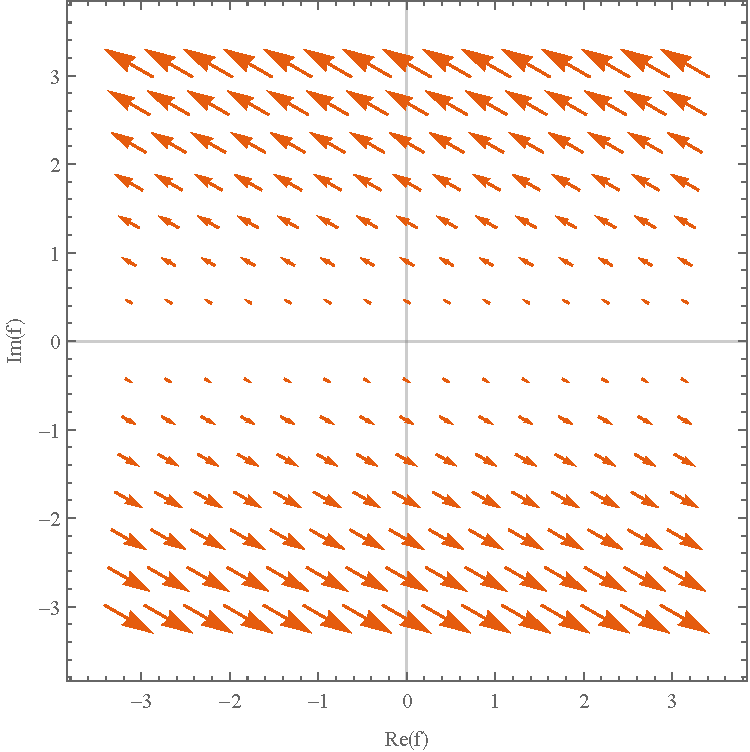
\includegraphics[width=0.5\textwidth]{fkvfield}
\caption{Orientation of $f(\vb{k})$} \label{fkvfield}
\end{figure}

\item If $\alpha > 2$ we can see from the expression of the energies $E'_{\pm}$ will never cancel and hence the two bands will never touch.

\end{enumerate}

\section{The Haldane Model}

\begin{enumerate}

\item Cells can be indexed by two integers $(i, j)$ where the $i$ index corresponds to the horizontal position and the $j$ to the vertical position. Then we write the orbitals $\ket{i, j, A}$ and $\ket{i, j, B}$ for $A$ and $B$ respectively. Then the Hamiltonian is given by:
\begin{align*}
H = \sum_{i, j} &t\Big(\op{i, j, B}{i, j, A} + \op{i, j+1, B}{i, j, A} + \op{i+1, j, B}{i, j, A}\Big)\\
+ &t_2 e^{i\varphi}\Big(\op{i, j + 1, A}{i,j, A} + \op{i, j - 1, A}{i,j, A} + \op{i - 1, j, A}{i,j, A}\Big) + \frac{M}{2}\op{i, j, A}\\
+ &t_2 e^{-i\varphi}\Big(\op{i, j + 1, B}{i,j, B} + \op{i, j - 1, B}{i,j, B} + \op{i - 1, j, B}{i,j, B}\Big) - \frac{M}{2}\op{i, j, B}\\
+ &h.c.
\end{align*}

\item The first line and it's Hermitian conjugate of the above definition of the Hamiltonian corresponds to the one studied in part one and we will denote it by $H_0$ which we already know can be expressed as $H_0 = \vb{h} \cdot \vb{\sigma}$. Now we study the two remaining lines of the Hamiltonian. The first one (resp. second one) corresponds to the contribution from clock-wise hoping on $A-A$ terms plus the staggered potential (resp. $B-B$ terms with the staggered potential). Which we can re-write as:
\[
\ket{i,j, A} \left(\frac{M}{2} + t_2 e^{i\varphi} \sum_{j = 1}^3 e^{i \vb{k} \cdot \vb{b_j}}\right) \bra{i, j, A} \mbox{~~and~~} \ket{i, j, B} \left(\frac{-M}{2} + t_2 e^{-i \varphi} \sum_{j = 1}^3 e^{i \vb{k} \cdot \vb{b_j}} \right)\bra{i, j, B}
\]
Then adding these with their conjugates will give:
\[
\begin{pmatrix}
\ket{i, j, A} & \ket{i, j, B}
\end{pmatrix} \begin{pmatrix}
2 \Re\left( t_2 e^{i \varphi} \sum_{j = 1}^3 e^{i \vb{k} \cdot \vb{b_j}} \right) + M & 0\\
0 & 2 \Re\left( t_2 e^{-i\varphi} \sum_{j = 1}^3 e^{i \vb{k} \cdot \vb{b_j}} \right) - M
\end{pmatrix}
\begin{pmatrix}
\bra{i, j, A}\\
\bra{i, j, B}
\end{pmatrix}
\]
Now from the properties:
\[
\Re(a b) = \Re(a)\Re(b) - \Im(a)\Im(b) \mbox{~~and~~} \Re(a) = \Re(a^\star) \mbox{~~and~~} \Im(a) = -\Im(a^\star)
\]
We can simplify the above (calling $a = t_2e^{i \varphi}$ and $b$ the sum):
\begin{align*}
&\begin{pmatrix}
\ket{i, j, A} & \ket{i, j, B}
\end{pmatrix} \begin{pmatrix}
2 \Re\left( ab \right) + M & 0\\
0 & 2 \Re\left( a^\star b \right) - M
\end{pmatrix}
\begin{pmatrix}
\bra{i, j, A}\\
\bra{i, j, B}
\end{pmatrix}
\\
=
&\begin{pmatrix}
\ket{i, j, A} & \ket{i, j, B}
\end{pmatrix} \begin{pmatrix}
2 \Re(a)\Re(b) - 2 \Im(a) \Im(b) + M & 0\\
0 & 2 \Re(a^\star) \Re(b) - 2 \Im(a^\star) \Im(b) - M
\end{pmatrix}
\begin{pmatrix}
\bra{i, j, A}\\
\bra{i, j, B}
\end{pmatrix}
\\
=
&\begin{pmatrix}
\ket{i, j, A} & \ket{i, j, B}
\end{pmatrix} \begin{pmatrix}
2 \Re(a)\Re(b) + (-2 \Im(a) \Im(b) + M)& 0\\
0 & 2 \Re(a) \Re(b) - (-2 \Im(a) \Im(b) + M) 
\end{pmatrix}
\begin{pmatrix}
\bra{i, j, A}\\
\bra{i, j, B}
\end{pmatrix}
\\
=
&\begin{pmatrix}
\ket{i, j, A} & \ket{i, j, B}
\end{pmatrix} \Bigg(2 Re(a) Re(b) \text{Id} + \Big(M - 2 \Im(a) \Im(b) \Big) \sigma_z \Bigg)
\begin{pmatrix}
\bra{i, j, A}\\
\bra{i, j, B}
\end{pmatrix}
\end{align*}
Hence now we write:
\[
\varepsilon_0(\vb{k}) = 2 \Re(a) \Re(b) = 2 \cos\varphi \sum_{j = 1}^3 \cos(\vb{k} \cdot \vb{b_j})
\]
As well as:
\[
d_z(\vb{k}) = M - 2 \Im(a) \Im(b) = M - 2 t_2 \sin(\varphi) \sum_{j = 1}^3 \sin(\vb{k} \cdot \vb{b_j})
\]
Then we define:
\[
\vb{d}(\vb{k}) = \vb{h}(\vb{k}) + d_z(\vb{k}) \vu{z}
\]
Which allows us to re-write:
\[
H = \sum_{\vb{k}} \begin{pmatrix}
\ket{\vb{k}, A} & \ket{\vb{k}, B}
\end{pmatrix}
\underbrace{\Big( \varepsilon_0(\vb{k}) \text{Id} + \vb{d}(\vb{k}) \cdot \vb{\sigma} \Big)}_{H_{\vb{k}}} \begin{pmatrix}
\bra{\vb{k}, A}\\
\bra{\vb{k}, B}
\end{pmatrix}
\]

\item We have immediately that the eigenvalues of $H_{\vb{k}}$ are going to be given by:
\[
E_{\pm\vb{k}} = \varepsilon_0(\vb{k}) \pm ||\vb{d}(\vb{k})||
\]
Hence we have that:
\[
\Delta E_{\pm \vb{k}} = E_{+\vb{k}} - E_{-\vb{k}} = 2 ||d(\vb{k})||
\]
Hence gaps close if and only if:
\[
2||\vb{d}(\vb{k})|| = 0 \Leftrightarrow ||\vb{h}(\vb{k})||^2 + d_z(\vb{k})^2 = 0 \Leftrightarrow \begin{cases}
||h(\vb{k})||^2 = 0\\
d_z(\vb{k})^2 = 0
\end{cases} \Rightarrow d_z(\vb{K}) = 0 \lor d_z(\tilde{\vb{K}}) = d_z(-\vb{K}) = 0
\]
Furthermore from the relation that we are given we have that:
\[
d_z(\vb{K}) = M + 3 t_2 \sin(\varphi)\sqrt{3} \mbox{~~and~~} d_z(\tilde{\vb{K}}) = M - 3 t_2 \sin(\varphi) \sqrt{3}
\]
Hence we will have conduction only along the lines (in the $(\sin\varphi, M)$ plane):
\[
M = - 3 t_2 \sqrt{3} \sin(\varphi) \mbox{~~and~~} M = 3 t_2 \sqrt{3} \sin(\varphi)
\]
Now denote by $s_+$ the sign of $d_z(\vb{K})$ and $s_-$ the sign of $d_z(\tilde{\vb{K}})$. Then the regions are plotted in Figure \ref{topregions}.

\begin{figure}
\centering
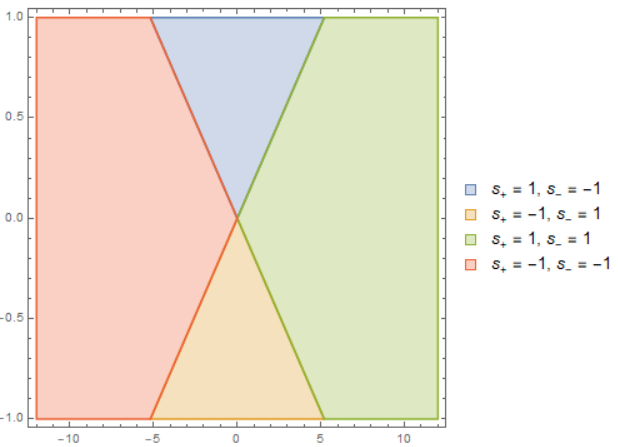
\includegraphics[width = 0.6\textwidth]{topregions}
\caption{Plot of the different insulating regions. The material has conductance along the two lines that cross the drawing. $s_+$ (resp. $s_-$ is the sign of $d_z(\vb{K})$ (resp. $d_z(-\vb{K})$).} \label{topregions}
\end{figure}

\item From the previous considerations the Chern number follows immediately from the equation given in the text. If you look at Figure $\ref{topregions}$ we will have $\nu = 2$ in the blue region (the upper cone), $\nu = -2$ in the yellow region (the lower cone) and $\nu = 0$ everywhere else.

\item 
As seen previously we have that:
\[
\Delta E_{\pm \vb{k}} = 2 || \vb{d}(\vb{k})|| = 2 | d_z(\vb{K}) |
\]
Now since we are at the boundary between two insulating phases of the Haldane insulator we have that $d_z(\vb{K})$ should be different for $y < 0$ and $y > 0$ hence we can write $d_z(\vb{K})_-$ for the value in $y < 0$ and identically with a plus for the $y > 0$ region. Then we have that:
\[
\Delta(y) = \Theta_{-y} d_z(\vb{K})_-  + \Theta_{y} d_z(\vb{K})_+ 
\]
Since however we are considering a physical system it might be more relevant to take a continuous smoothing of the $\Theta$ distribution. Hence we could also take:
\[
\Delta(y) = f(d_z(\vb{K})_-, d_z(\vb{K})_+) \mbox{~~where~~} f(m, p) = \frac{m e^{cr} + p e^{ry}}{e^{cr} + e^{ry}}
\]
With $r$ being a parameter determining the sharpness of the transition and $c$ determining the value of the intersect $\Delta = 0$. When $p$ and $m$ have opposite sign it is logical to choose the origin of the axis such that the intersect $\Delta = 0$ happens at $y = 0$. This is obtained for $c = \frac{1}{r}\log(-\frac{b}{a})$. 

\item In order to linearize we can use the following simplification: $\cos(\vb{q} \cdot \vb{b_j}) = 1 + \mathcal{O}(||\vb{q}||^2)$ and $\sin(\vb{q} \cdot \vb{b_j}) = \vb{q} \cdot \vb{b_j} + \mathcal{O}(||\vb{q}||^3)$. Then we can re-write:
\[
\varepsilon_0(\vb{K} + \vb{q}) = 2\cos\varphi \sum_{j = 1}^3 \cos(\vb{K} \cdot \vb{b_j} + \vb{q} \cdot \vb{b_j}) = 2 \cos\varphi \sum_{j = 1}^3 \Big( \cos(\vb{K} \cdot \vb{b_j}) \cdot 1 - (\vb{q} \cdot \vb{b_j}) \sin(\vb{K} \cdot \vb{b_j})  \Big)
\] 
Now we can simplify this as follows:
\[
\varepsilon_0(\vb{K} + \vb{q}) = \underbrace{\varepsilon_0(\vb{K})}_{-3 \cos \varphi} - 2 \cos \varphi \, \vb{q} \cdot \underbrace{\sum_{j = 1}^3 \vb{b_j} \sin(\vb{K} \cdot \vb{b_j})}_{= 0}
\]
Similarly we get:
\begin{align*}
d_z(\vb{K} + \vb{q}) &= M - 2 t_2 \sin(\varphi) \sum_{j = 1}^3 (\vb{q} \cdot \vb{b_j})\cos(\vb{K} \cdot \vb{b_j}) + \sin(\vb{K} \cdot \vb{b_j}) \\
&= d_z(\vb{K}) - 2 t_2 \sin(\varphi) \vb{q} \cdot \underbrace{\sum_{j = 1}^3 \vb{b_j} \cos(\vb{K} \cdot \vb{b_j})}_{= 0} = d_z(\vb{K})
\end{align*}
Then from the previous linearization of $\vb{h}$ we already have:
\[
d_x(\vb{K} + \vb{q}) = \frac{3 d t}{2} q_x \mbox{~~and~~} d_y(\vb{K} + \vb{q}) = \frac{3 d t}{2} q_y
\]
So in total we obtain:
\[
\varepsilon_0(\vb{K}+\vb{q}) = -3 \cos \varphi \mbox{~~and~~} d_x(\vb{K} + \vb{q}) = \frac{3 d t}{2} q_x \mbox{~~and~~} d_y(\vb{K} + \vb{q}) = \frac{3 d t}{2} q_y \mbox{~~and~~} d_z(\vb{K} + \vb{q}) = d_z(\vb{K})
\]
Which gives the following Hamitlonian:
\[
H_1(\vb{q}) = \begin{pmatrix}
- 3 \cos\varphi + d_z(\vb{K}) & \frac{3 dt}{2}(q_x - i q_y)\\
\frac{3 dt}{2}(q_x + i q_y)  & - 3 \cos \varphi - d_z(\vb{K})
\end{pmatrix}
\]
\item We introduce the Fermi velocity:
\[
v_F = \frac{3 d t}{2\hbar}
\]
Then the above Hamiltonian can be re-written (where $\vb{p} = \hbar \vb{q}$):
\[
H_1(\vb{q}) = -3 \cos\varphi \text{Id} + v_F(p_x \sigma_x + p_y \sigma_y) + d_z(\vb{K}) \sigma_z
\]
To go back to the real space Hamiltonian it suffices to take a Fourier transform of the expression above. From quantum mechanics we know that $\vb{p} = -i\hbar \grad_{x, y, z}$. Furthermore since we can define the Hamiltonian up to a constant we can remove the first term and we are left with the required from of the Hamiltonian. 

\item We have that (taking $\psi$ to be the prefactor of $\psi_{q_x}$):
\begin{align*}
(H_1 \psi_{q_x}(x, y))^{\pm} &= \Big[- i \hbar v_F (\partial_x \mp i \partial_y) \pm \Delta(y)\Big] \psi = \Big[- i \hbar v_F(iq_x \mp \frac{i}{\hbar v_F} \Delta(y)) \pm \Delta(y)\Big]\psi\\
&= \Big[ \hbar v_F q_x \mp  \Delta(y) \pm \Delta(y) \Big] \psi = \hbar v_F q_x \psi
\end{align*}
So:
\[
H_1 \psi_{q_x}(x,y) = \hbar v_F q_x \psi_{q_x}(x, y)
\]

\item We have that:
\[
|\psi|^2 = 2e^{\frac{2}{\hbar v_F} \int_0^y \Delta(y') \dd y'}
\]
Now notice that from the construction of $\Delta(y')$:
\[
\Delta(y) = f(d_z(\vb{K})_-, d_z(\vb{K})_+) \mbox{~~where~~} f(m, p) = \frac{m e^{cr} + p e^{ry}}{e^{cr} + e^{ry}}
\]
That we have multiple possible cases. If $\text{sign}(d_z(\vb{K})_-) = \text{sign}(d_z(\vb{K})_+)$ then the amplitude will diverge on one side at least. If $d_z(\vb{K})_+ > 0$ and $d_z(\vb{K})_- < 0$ then the amplitude will diverge on both sides. However if $d_z(\vb{K})_+ < 0$ and $d_z(\vb{K})_- > 0$ then the amplitude will converge and in fact the wavefunction will be square integrable as is required by quantum mechanics. This shows mutliple points:
\begin{enumerate}
\item A solution can exist only along one direction of the transition, which gives the chirality of the edge state.
\item Second of all an edge state is called an edge state because the wavefunction will be strongly localized around $y = 0$.
\end{enumerate}
\end{enumerate}
If we take the sharp heavyside transition the integral is easy to compute and gives:
\[
\int_0^y \Delta(y') \dd y' = d_z(\vb{K})_{\text{sign}(y)} |y|
\]
If we place ourselve in the only converging case we can write:
\[
\int_0^y \Delta(y') \dd y' = d_z(\vb{K})_{\text{sign}(y)} |y| = - |d_z(\vb{K})_{\text{sign}(y)} y| 
\]
And hence the amplitude has a simple decaying exponential expression.

\begin{figure}
\centering
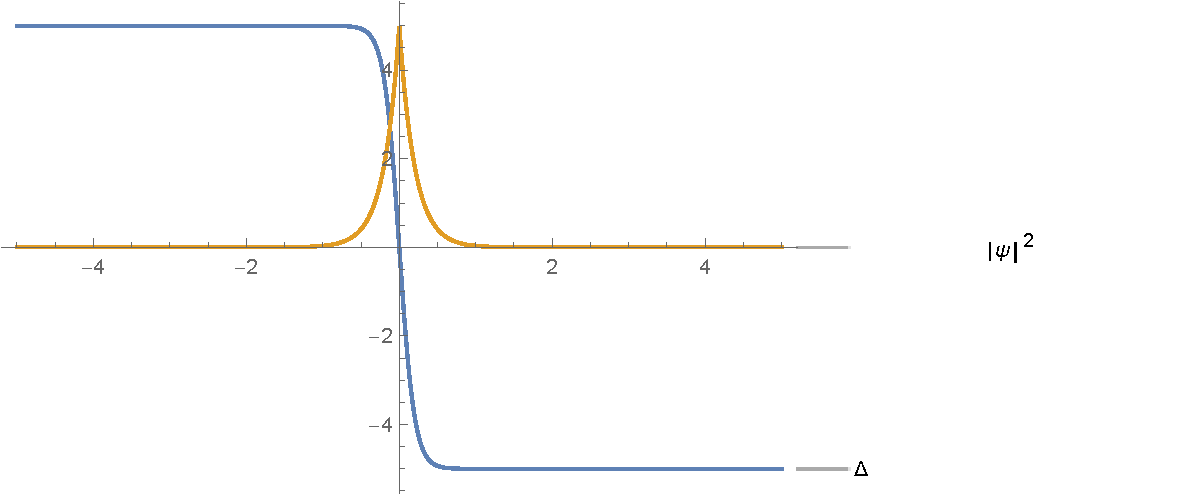
\includegraphics[width=0.6\textwidth]{edgestate}
\caption{Plot of the amplitude of a valid edge state together with the corresponding $\Delta$ function.}
\end{figure}

\end{document}